\documentclass[10pt]{beamer}
% Class options include: notes, notesonly, handout, trans,
%                        hidesubsections, shadesubsections,
%                        inrow, blue, red, grey, brown

% Theme for beamer presentation.
%\usepackage{beamerthemesplit} 
\usepackage{amsmath}
\usepackage{multirow,booktabs}
\usepackage{graphicx}
\usepackage{subfig}
\usepackage{amssymb}
\usepackage{amsthm}
%\usepackage{enumitem}
%\usepackage{mathtools}
\usepackage{setspace} % Needed for interline space of the texts. 
%\usepackage{tikz}
%\usepackage{caption}
\usepackage{verbatim}
\usepackage{rotating}
\usepackage{color}
\usepackage{setspace}
\usepackage{numprint}
\theoremstyle{plain}

%\newtheorem{proposition}[theorem]{Proposition}[section]

\usetheme{Berlin}
%\useinnertheme{rectangles}
%\useoutertheme{infolines}
\usecolortheme{dove}
% Other themes include: beamerthemebars, beamerthemelined, 
%                       beamerthemetree, beamerthemetreebars  

\title{\sc Housing Prices and Crime Rates}    % Enter your title between curly braces
\author{\sc Debanjan Mitra}
\institute{\sc Indian Institute of Management Udaipur}      % Enter your institute name between curly braces
\date{}                    % Enter the date or \today between curly braces

\begin{document}

% Creates title page of slide show using above information
\begin{frame}
  \titlepage
\end{frame}



\begin{frame}
\frametitle{\sc The Problem}
	A community in the Philadelphia area is interested in how crime rates affect property values. If low crime rates increase property values, the community might be able to cover the costs of increased police protection by gains in tax revenues from higher property values. 
	\vskip 0.2in 
	
	If the community can cut its crime rate from 30 down to 20 per 1000 population, what sort of change might it expect in the property values of a typical house? 
\end{frame}


\begin{frame}
\frametitle{\sc The Data}
	\begin{itemize}
		\item The city council has data for 110 communities in Pennsylvania near Philadelphia
		\item For each community, the data has information on the following: \\
		\textcolor{orange}{\textit{HousePrice}}: average house price during the most recent year \\
		\textcolor{orange}{\textit{CrimeRate}}: Rate of crimes per 1000 population \\
		\textcolor{orange}{\textit{MilesPhila}}: Miles to Philadelphia \\
		\textcolor{orange}{\textit{PopChg}}: Change in population, as a percentage \\
		\textcolor{orange}{\textit{Name}}: Name of the community \\
		\item We shall use data for 98 communities, as rest (i.e., 12 communities) have ``NA'' values for some of the variables
		\item We shall use the first two variables: \textcolor{orange}{\textit{HousePrice}} and \textcolor{orange}{\textit{CrimeRate}}
    \end{itemize}		
\end{frame}


\begin{frame}
\frametitle{\sc A First Look at the Data}
	\begin{figure}[!ht]
		\centering
		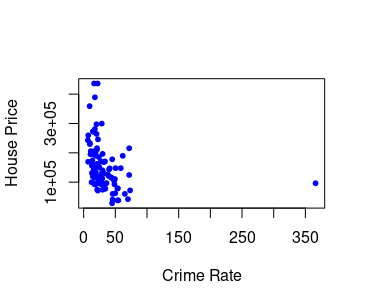
\includegraphics[scale=0.9]{figs8/scatter-all.png}
		%\caption{}
	\end{figure}
\end{frame}

\begin{frame}
\frametitle{\sc The Outlier}
	\begin{itemize}
		\item This odd community (\underline{Center City, Philadelphia})  is an outlier on the horizontal axis \textcolor{orange}{\textit{CrimeRate}}, but is not unusual on the vertical axis (House Price)
		\item If we fit a least square regression line to this data, the outlier will pull the regression fit toward itself
		\item \textcolor{red}{As the sum of \underline{squared deviations} from the regression is minimized in least squares, observations that are far from the fit may have substantial influence on the location of the line}
		\item The size of the impact depends upon \underline{\textcolor{blue}{the leverage}} of the outlying value
    \end{itemize}		
\end{frame}

\begin{frame}
\frametitle{\sc The Outlier}
	\begin{itemize}
		\item Leverage measures how unusal an observation is along the x-axis (here, the \textcolor{orange}{\textit{CrimeRate}})
		\item \textcolor{red}{In simple linear regression, the leverage of the $i$-th observation is defined as
		\[
		Leverage = h_i = \frac{1}{n} + \frac{(X_i - \bar{X})^2}{SS_X},
		\]
		where $SS_X$ is the sum of squared deviations about the mean of $X$}
		\item The value of leverage is in the range 
		\[
		\frac{1}{n} \leq h_i \leq 1
		\]
		\item Here, Center City, Philadelphia is a highly leveraged observation (leverage = 0.82)
    \end{itemize}		
\end{frame}

\begin{frame}
\frametitle{\sc Fitting a Simple Regression Model}
	\begin{itemize}
		\item First, let us fit a simple regression model to the data
		\item \textcolor{orange}{\textit{HousePrice}} is the response, and \textcolor{orange}{\textit{CrimeRate}} is the predictor
	\end{itemize}
    \begin{table}[hptb]
	\scriptsize
	\caption{\small Simple Regression Model for the Data}
	\begin{center}
		\begin{tabular}{ c c c c c} 
			\toprule
			& Estimate & Std. Error & $t$-value & $p$-value \\
			\midrule
			Intercept & 173116.4 & 10486.5 &  16.509  & $<$ 2e-16 \\
			CrimeRate & -567.7   & 210.9   &  -2.692  & 0.00837 \\ 
			\bottomrule
		\end{tabular}
		\end{center}
\end{table}
\end{frame}

\begin{frame}
\frametitle{\sc The Fitted Line and the Data}
	\begin{figure}[!ht]
		\centering
		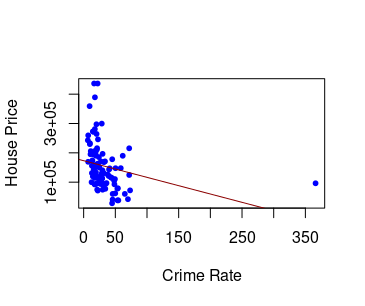
\includegraphics[scale=0.9]{figs8/scatter-all-reg.png}
		%\caption{}
	\end{figure}
\end{frame}

\begin{frame}
\frametitle{\sc Residual Plot}
    \begin{figure}[!ht]
		\centering
		\includegraphics[scale=0.9]{figs8/residual.png}
		%\caption{}
	\end{figure}
\end{frame}

\begin{frame}
	\frametitle{\sc Distribution of Residuals}
	\begin{itemize}
		\item The overall distribution of the residuals is skewed to the right
    \end{itemize}	
    \begin{figure}[!ht]
		\centering
		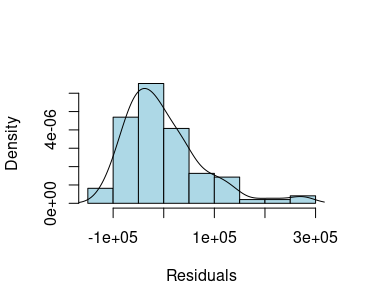
\includegraphics[scale=0.8]{figs8/residuals-density.png}
		%\caption{}
	\end{figure}	
\end{frame}

\begin{frame}
\frametitle{\sc The QQ Plot}
	\begin{itemize}
		\item The Quantile-Quantile (QQ) plot of the residuals shows that there is a problem with normality assumption, although the plot is dominated by the outlier
    \end{itemize}	
    \begin{figure}[!ht]
		\centering
		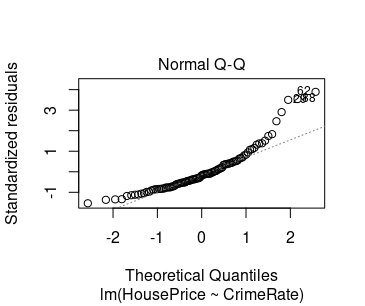
\includegraphics[scale=0.8]{figs8/QQ-full.png}
		%\caption{}
	\end{figure}	
\end{frame}

\begin{frame}
\frametitle{\sc Handling the Outlier}
	\begin{itemize}
		\item It is clear from the above analyses that the outlier is affecting the model quite  strongly
		\item We need to handle the outlier before further analyses
		\item Let us repeat the analyses deleting the outlier
    \end{itemize}	
\end{frame}

\begin{frame}
\frametitle{\sc A Model Without The Outlier}
    \begin{figure}[!ht]
		\centering
		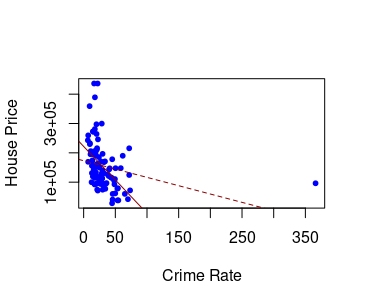
\includegraphics[scale=0.9]{figs8/reg-minus-outlier.png}
		%\caption{}
	\end{figure}
\end{frame}

\begin{frame}
\frametitle{\sc A Model Without The Outlier}
	\begin{itemize}
		\item Delete the outlier, and fit the simple regression model as before
	\end{itemize}
    \begin{table}[hptb]
	\scriptsize
	\caption{\small Simple Regression Model for the Data}
	\begin{center}
		\begin{tabular}{ c c c c c} 
			\toprule
			& Estimate & Std. Error & $t$-value & $p$-value \\
			\midrule
			Intercept & 221775.6  & 15059.6  & 14.727 & $<$ 2e-16 \\
            CrimeRate & -2281.6   &   450.6  & -5.063 & 2.02e-06 \\
			\bottomrule
		\end{tabular}
		\end{center}
\end{table}
\end{frame}


\begin{frame}
\frametitle{\sc Comparison: Two Models}
	\begin{itemize}
		\item The regression model with the outlier in the data is
		\textcolor{blue}{\[
		House Price = 173116.4 - 567.7 \times Crime Rate
		\]}
		\item The regression model without the outlier in the data is
		\textcolor{blue}{\[
		House Price = 221775.6 - 2281.6 \times Crime Rate
		\]}
		\item Without the outlier, the slope of the regression line is almost four times the slope of the previous line
		\item The change in the regression line is dramatic, and so is the change in the estimated effect of \textcolor{orange}{\textit{Crime Rate}} on \textcolor{orange}{\textit{House Price}}
	\end{itemize}
\end{frame}

\begin{frame}
\frametitle{\sc The New Fit}
    \begin{figure}[!ht]
		\centering
		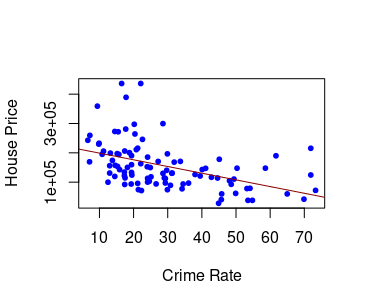
\includegraphics[scale=0.7]{figs8/scatter-reg-new.png}
		%\caption{}
	\end{figure}
\begin{itemize}
\item While the fit has definitely improved, but the plotted points seem to show a nonlinear pattern
\end{itemize}	
	
\end{frame}


\begin{frame}
\frametitle{\sc New Residual Plot}
    \begin{figure}[!ht]
		\centering
		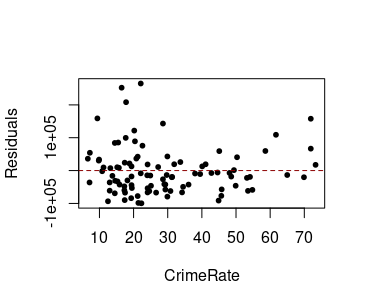
\includegraphics[scale=0.7]{figs8/residual-new.png}
		%\caption{}
	\end{figure}
\begin{itemize}
\item Residuals also indicate nonlinearity; implies some transformation of the predictor will be useful
\end{itemize}	
\end{frame}


\begin{frame}
\frametitle{\sc New QQ Plot}
    \begin{figure}[!ht]
		\centering
		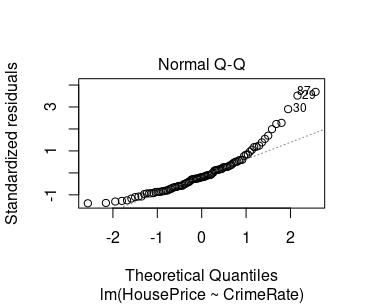
\includegraphics[scale=0.7]{figs8/QQ-new.png}
		%\caption{}
	\end{figure}
\begin{itemize}
\item The QQ plot clearly shows positive skewness of the residuals (i.e., many small negative residuals, and few large positive residuals)
\end{itemize}
\end{frame}

\begin{frame}
	\frametitle{\sc Impact of Crime Rate}
	\begin{itemize}
		\item The regression model with Center City in the data is
		\textcolor{blue}{\[
		House Price = 173116.4 - 567.7 \times Crime Rate
		\]}
		\item The regression model without Center City in the data is
		\textcolor{blue}{\[
		House Price = 221775.6 - 2281.6 \times Crime Rate
		\]}
		\item Consider a 10-point drop in \textcolor{orange}{\textit{CrimeRate}}
		\item With Center City, the increase in \textcolor{orange}{\textit{HousePrice}} is $10 \times \$567.7 \approx \$5700$ per house
		\item Without Center City, the increase in \textcolor{orange}{\textit{HousePrice}} is $10 \times \$2281.6 \approx \$23000$ per house
		\item \textcolor{red}{Caution: The data for house prices are from sales of current year only - may not be representative of the actual sales}
	\end{itemize}
\end{frame}

\begin{frame}
\frametitle{\sc Scatterplot Smoothing}
    \begin{figure}[!ht]
		\centering
		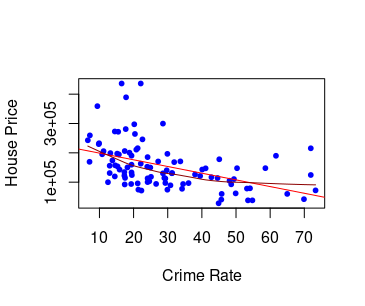
\includegraphics[scale=0.8]{figs8/scatter-smooth.png}
		%\caption{}
	\end{figure}
\begin{itemize}
\item The nonlinear relationship is clear!
\end{itemize}
\end{frame}

\begin{frame}
\frametitle{\sc Fitting a Transformed Model}
	\begin{itemize}
	\item We fit the reciprocal model to this data, that is, 
\textcolor{blue}{\[
HousePrice = \alpha + \beta \times (1/CrimeRate)
\]}
	\item With the estimated coefficients, the model is 
\textcolor{blue}{\[
HousePrice  = 92256 + 1350722 \times (1/CrimeRate)
\]}
	\item To see if the new transformed model is better on this data, look at the residuals - a plot of the residuals against \textcolor{orange}{\textit{CrimeRate}}, and the QQ plot of the residuals
	\end{itemize}
\end{frame}

\begin{frame}
\frametitle{\sc Residual Plot for The Transformed Model}
    \begin{figure}[!ht]
		\centering
		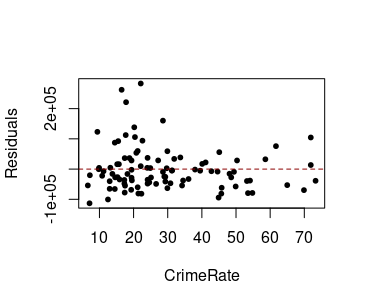
\includegraphics[scale=0.9]{figs8/residuals-recip.png}
		%\caption{}
	\end{figure}
\end{frame}

\begin{frame}
\frametitle{\sc Impact of Crime Rate: The Transformed Model}
	\begin{itemize}
	\item \textcolor{magenta}{Change in fit($CrimeRate$ 20 to 10) $= \frac{13350722}{10} - \frac{13350722}{20} = \$67536$}
	\item \textcolor{magenta}{Change in fit($CrimeRate$ 30 to 20) $= \frac{13350722}{20} - \frac{13350722}{30} = \$22512$}
	\item The fitted model flatens out as \textcolor{orange}{\textit{CrimeRate}} increases
	\item That is, increase in \textcolor{orange}{\textit{CrimeRate}} has a big effect on house prices for smaller crime rates; the effect is smaller when the crime rates are larger
	\end{itemize}
\end{frame}

\begin{frame}
\frametitle{A Word of Caution}
	\begin{itemize}
	\item Do crime rates affect house prices, or is it the other way round? 
	\item Maybe some third factor, like education? (\textcolor{blue}{lurking variable})
	\item Regression, like correlation, is based on association
	\item In general, it cannot deduce cause and effect relationship (unless it is based on an experimental design)
	\end{itemize}
\end{frame}

\end{document}
